\documentclass[conference]{IEEEtran}
\usepackage{amsmath,amssymb,graphicx}
\usepackage{listings}
\usepackage[dvipsnames]{xcolor}
\lstset{
      language=C++,
      backgroundcolor=\color{black!5}, % set backgroundcolor
      aboveskip=3mm,
  belowskip=3mm,
  showstringspaces=false,
  columns=flexible,
  basicstyle=\fontsize{9}{12}\ttfamily,
  numbers=left,                 
  numbersep=5pt,               
  showspaces=false,                
  showstringspaces=false,
  showtabs=false,
  numberstyle=\tiny\color{black},
  keywordstyle=\color{blue},
  commentstyle=\color{ForestGreen},
  stringstyle=\color{mauve},
  breaklines=true,
  breakatwhitespace=true,
  tabsize=3
  }



% nice symbols for real and complex numbers
\newcommand{\R}[0]{\mathbb{R}}
\newcommand{\C}[0]{\mathbb{C}}
% bold paragraph titles
\newcommand{\mypar}[1]{{\bf #1.}}

\begin{document}

\title{Evaluating tensor cores}


\author{\IEEEauthorblockN{John Carlsson, Cyprien Touron Decourteix}
\IEEEauthorblockA{Department of Computer Science\\
 University of Salerno\\
 Italy}
}

\maketitle

\begin{abstract}\label{sec:abstract}
In this paper we evaluate the use of tensor cores in CUDA through experiments to get a better 
understanding of high performance computing. The goal is to compare the time 
to calculate a matrix multiplication addition and analyze the impact of tensor cores compared to CPU and GPU
usage. Finally we will present the results of the benchmarking and show that utilizing tensor cores 
provides significant improvements when measuring the computational time.

\end{abstract}

\section{Introduction}\label{sec:intro}


Over the past decade, the increasing demand for deep learning and AI applications has
fueled the need for highly efficient tensor operations. Traditional GPU architectures are powerful but 
are often limited in their ability to fully exploit the potential of 
tensor computations due to the reliance on higher-precision floating-point arithmetic. 
tensor cores address this limitation by leveraging mixed-precision arithmetic, combining 
high throughput with reduced precision.

tensor cores, introduced in NVIDIA's Volta architecture and further enhanced in 
subsequent architectures such as Turing and Ampere, have revolutionized the performance of 
tensor computations on GPUs. These specialized hardware units offer significant speedups 
by providing native support for low-precision tensor operations, 
specifically matrix multiplications and convolutions. 
The purpose of this project report is to present an evaluation of tensor cores,
exploring their capabilities compared to CPU and GPU based computation.

We aim to evaluate tensor cores using the Matrix Multiplication Accumulate (MMA) with various 
workloads and compare the results to the CPU and GPU performances. 

By conducting this comprehensive evaluation, we aim to provide insights into the capabilities and 
limitations of tensor cores. Additionally, the findings from this study will contribute to the 
broader understanding of GPU acceleration techniques for tensor operations and their potential 
impact on high-performance computing.

\subsection{Motivation}\label{sec:Motivation}

The MMA operation plays a critical role in accelerating various computational tasks.
It involves three matrices and is fundamental within many computational domains, 
such as deep learning, scientific simulations, and image processing. However, performing MMA 
efficiently and at scale is difficult due to the intensity of the operation. 

The difficulties that arise when trying to implement a fast version of MMA are due to 
a combination of factors including memory access patterns, 
computational intensity, hardware limitations, and optimization trade-offs.

The objective of this paper is to provide valuable insights for optimizing MMA computations
and facilitate the adoption of tensor cores as a powerful tool for accelerating MMA 
operations in comparison to CPU and GPU. Our contributions will be as follows:

\begin{itemize}
  \item Measure the speedup achieved by tensor cores and explore how 
  performance scales with the size of the matrices.

  \item Compare the performance of tensor cores with CPU and GPU implementations of MMA 
  using different matrix sizes and precision settings.
  
  \item Analyze the impact of data precision on the performance of tensor cores and 
  investigate the trade-offs between accuracy and computation time.
  
  \item Provide insights into the limitations and challenges of tensor cores, 
  including memory constraints, data dependencies, and scalability issues.
  
  \end{itemize}
  
  \section{Background}\label{sec:background}
  

  Tensor cores are specialized hardware units introduced in NVIDIA GPUs that are designed to accelerate matrix computations, 
  specifically matrix multiplications and convolutions. They leverage mixed-precision arithmetic, 
  combining high throughput with reduced precision to achieve significant speedups in tensor operations.
  
  The key feature of tensor cores is their ability to perform mixed-precision operations using 
  half-precision floating-point (FP16) data types. By using FP16, tensor cores can process a larger 
  number of elements simultaneously, leading to improved throughput at the cost of accuracy.\cite{precision_FMA} 
  
  Tensor cores operate on 4x4 matrix tiles, performing matrix multiplication and accumulation (MMA) 
  operations. These operations are highly parallel and can be efficiently executed on tensor cores. 
  By exploiting the parallelism of tensor cores and their ability to process multiple elements 
  simultaneously, significant performance gains can be achieved compared to traditional GPU 
  implementations.

  The tensor operations are warp size, this means that each tensor instruction must work on the same 
  data within the same warp.
  
  \subsection{Matrix Multiplication Accumulate (MMA)}\label{sec:mma}
  
  Matrix Multiplication Accumulate (MMA) is a key operation in many computational tasks, including deep 
  learning, scientific simulations, and image processing. It involves three matrices: two input matrices 
  (A and B) and an output matrix (C). The operation computes the matrix product of A and B and accumulates 
  the result into C.
  
  Mathematically, the MMA operation can be defined as follows:
  
  \[ D \leftarrow \alpha \cdot A \cdot B + \beta \cdot C \]
  
  where A is an m x k matrix, B is a k x N matrix, C is an m x N matrix, and $\alpha$ and $\beta$ are scalar coefficients.
  
  The MMA operation is computationally intensive and can benefit greatly from hardware acceleration. 
  Tensor cores, with their ability to efficiently perform MMA operations, offer a promising solution 
  for accelerating this operation.
  
  
  \section{Code}
  In this section we present the main part of the code. The code shown is the computational part. 
  We show here the CUDA code and the tensor code.

  \subsection{CPU code}\label{sec:CPUCode}
  We implement a CPU version of the MMA operation to have a reference to verify our computation results.
  The CPU code is an implementation of the MMA operation that uses the following optimizations:
  \begin{enumerate}
    \item Tiling
    \item Tarallelisation using OpenMP
    \item Compiler vectorisation for AVX512 using OpenMP
    \item Compiler optimization flags
  \end{enumerate}


  \subsection{CUDA code}\label{sec:CudaCode}
  We implemented multiple versions of the matrix multiplication and addition with CUDA to
  study the effect of multiple optimizations techniques. For each implementation, 
  the code is heavily simplified to keep the essence. For full code, see appendix.

  \subsubsection[short]{Basic MMA in CUDA}
  The MMA implement in CUDA is very basic as it uses the base formula of a matrix multiplication
  and addition and assign one thread per each element of the output matrix.\cite{Cpp_programming}


  \subsubsection[short]{MMA with shared Memory}
  This MMA implement uses shared memory to optimize global memory acces count. The multiplication operation 
  is done using tiling with the size of the tile matching the size of the block. For each tile, within
  a same block, each threads load a single element of the tile to the shared memory. 
  \begin{lstlisting}
  __global__ void MMACudaShared(float *out, float *A, float *B, float *c, int n)
  {   
      sum = c[...];
      for (tileNum = 0; tileNum < n/TILE_SIZE; tileNum++){
          a_shared[...] = A[...];
          b_shared[...] = B[...];
          __syncthreads();
          for (int k = 0; k < TILE_SIZE; k++)
          {sum += a_shared[...] * b_shared[...]; }
      }
      out = sum;
  }   
  \end{lstlisting}

  \subsubsection[short]{Mixed precision MMA}
  The CUDA API provides the posibility to work with floating point numbers of half the size of regular 32 bits floats.
  Mixed computation works with A and B being half precision floats matrices and C and D being float matrices.
  We made two versions of this MMA Mixed precision operation based on the MMA shared memory implementation. One version
  convert halfs to float before doing the computation to see the effect on bandwidth and the other does the conversion after.
  We also tried a third implementation using the CUDA FMA instruction but  
  \begin{lstlisting}
  __global__ void MMACudaMixedA(float *out, half *A, half *B, float *c, int n)
  {   
      ...
          for (int k = 0; k < TILE_SIZE; k++)
          sum += (float)a_shared[...] * (float)b_shared[...]; }
      ...
  }
  __global__ void MMACudaMixedB(float *out, half *A, half *B, float *c, int n)
  {   
      ...
          for (int k = 0; k < TILE_SIZE; k++)
          sum += (float)(a_shared[...]+ b_shared[...] ) ; }
      ...
  }
  \end{lstlisting}
  \subsubsection[short]{Thread coarsening Mixed precision MMA}
  The space gained in the shared memory is not enough to double the tile size of the shared memory. We wanted 
  to maximize the usage of the shared memory to reduce the amount of time each thread has to wait for the memory
  to arrive to the shared memory between each operation. This operation is based on Mixed precision implementation.
  This is done by making the threads working on computing multiple elements of the output matrices (see figure \ref{fig:thread-coars}). In this case
  NUMTHREADS is the amount of elements each thread has to compute.
  \begin{figure}[h]
    \centering
    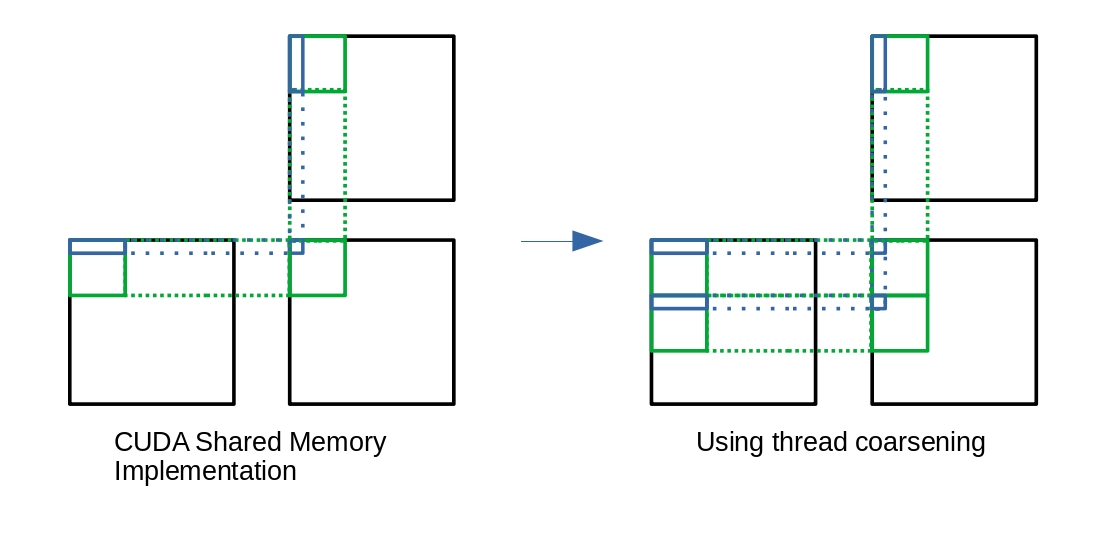
\includegraphics[scale=0.2]{figures/threadCoarsening.png}
    \caption{Performance Comparison total time with deallocation}
    \label{fig:thread-coars}
  \end{figure}

  \begin{lstlisting}
  __global__ void MMACoarsening(float *out, half *A, half *B, float *c, int n)
  {   
      Out accs[NUMTHREADS];
      for (subthread = 0; subthread < NUMTHREADS; subthread++)
          accs[subthread] = c[(row + TILE_SIZE * subthread)*n + col];
      for (tileNum = 0; tileNum < n/TILE_SIZE; tileNum++){
          for (subthread = 0; subthread < NUMTHREADS; subthread++)
              a_shared[subthread][...] = A[...];
          b_shared[...] = B[...];
          __syncthreads();
          for (int k = 0; k < TILE_SIZE; k++)
              for (subthread = 0; subthread < NUMTHREADS; subthread++)
              {accs[subthread]m += (float)a_shared[subthread][...] * (float)b_shared[...]; }
      }
      for (subthread = 0; subthread < NUMTHREADS; subthread++)
        out[...] = accs[subthread];
  }
  \end{lstlisting}
  
  
  \subsection{tensor code}\label{sec:tensorCode}
  The tensor code is implemented using the WMMA API,  Warped matrix multiplication addition,
  library. We are working in our case with 16x16x16 fragments with a row-major memory layout.
  \begin{lstlisting}
  using namespace wmma
  __global__ void mat_mul_add_tensor(half *a, half *b, float *C, float *d, int N){
    // Declare the fragments
    fragment<matrix_a, ...> a_frag;
    fragment<matrix_b, ...> b_frag;
    fragment<wmma::accumulator, ..., float> c_frag;
    load_matrix_sync(c_frag, C, N, mem_row_major);
    // Loop over k
    for (int i = 0; i < N; i += WMMA_K){
      load_matrix_sync(a_frag, a, N);
      load_matrix_sync(b_frag, b, N);
      // Perform the matrix multiplication
      mma_sync(c_frag, a_frag, b_frag, c_frag);
    }
    store_matrix_sync(d, c_frag, N, mem_row_major);
  }
  \end{lstlisting}

  We tried to shared memory and an implementation with the cuBLASs library but we had terrible 
  accuracy results and did not had time to find a solution to fix them. 

  \section{Experimental Setup}\label{sec:experimental-setup}
  
  In this section, we describe the experimental setup used to evaluate 
  tensor cores and compare their performance with CPU and GPU implementations of MMA.
  We did a multitude of tests with different parameters to see how performance scale over matrix size.

  We used square matrices with the sizes of NxN where N starts at 32 and is doubled up to 8192.

  \begin{table}[h]
    \caption{Size of N}
  \centering
    \begin{tabular}{|c|}
    \hline
    32 \\
    \hline
    64 \\
    \hline
    128 \\
    \hline
    256 \\
    \hline
    512 \\
    \hline
    1024 \\
    \hline
    2048 \\
    \hline
    4096 \\
    \hline
    8192 \\
    \hline

    \end{tabular}
  \end{table}

  we conducted single-run comparisons to measure the computation error and then 100 runs to get a better average for time.
  Each implementation works on the same input matrices that are made of float elements that are initialised with random values between 0 and 1
  and are not allocated in an alligned way. The cpu implementation will allign the matrices before the computation and each mixed precision implementation will do a CPU pass do the conversion they need
  before sending the data to the GPU, these conversions and memory managements are not mesured in the computation 
  measurements, however it is taken in account for the total operation execution time.

  \subsection{Hardware Configuration}\label{sec:hardware-configuration}
  
  The experiments were conducted on a system equipped with an NVIDIA GPU, the NVIDIA Quadro 4000 RTX.
  The specifics are shown in table \ref{GPU}.
  
  \begin{table}[htbp]
  \caption{GPU Specifications\cite{Voltatuningguide}}
  \centering
  \label{GPU}
    \begin{tabular}{|c|c|}
    \hline
    GPU Model & NVIDIA Quadro 4000 RTX \\
    \hline
    CUDA cores & 2304 \\
    \hline
    Tensor cores & 288 \\
    \hline
    Memory interface & 256-bit \\
    \hline
    CUDA version & 11.8 \\
    \hline
    Compute capability & 7.5 \\
    \hline
    Shared memory size & 64 kb \\
    \hline
    
  \end{tabular}
  \end{table}
  
  \subsection{Software Configuration}\label{sec:software-configuration}
  
  The experiments were conducted using the following software tools and frameworks:
  
  \begin{itemize}
    \item CUDA Toolkit version 11.8
    \item WMMA
    \item C++17 compiled with g++ 11.3.0
  \end{itemize}
  \subsection{implementations parameters}
  Each of our CUDA implementations, except for the thread coarsening one uses threadblocks of 32x32.
  The thread coarsening version is executed twice with a different value (2 and 3) for NUMTHREADS. This
  mean that the thread coarsening version will be allocating twice and a third of the amount of threads
  by the other CUDA implementations. The tensor implementation work block that handle 4x4 matrices of
  16x16 elements, therefore the block size is 128x4.

  \subsection{Benchmarking Methodology}\label{sec:benchmarking-methodology}
  
  To evaluate the performance of tensor cores, we performed a series of experiments using different 
  matrix sizes and precision settings. For each experiment, we measured the execution time of the 
  MMA operation for CPU, GPU without tensor cores, and GPU with tensor cores implementations.
  
  We varied the matrix sizes from small to large to analyze the impact of matrix dimensions on 
  performance. Additionally, we tested different precision settings, including full precision (FP32)
  and mixed precision (FP16 and FP32).
  
  To ensure accurate measurements, we repeated each experiment multiple times and calculated 
  the average execution time. We also recorded the peak memory usage during each experiment to 
  analyze the memory requirements of tensor cores.
  
  \section{Results and Analysis}\label{sec:results-analysis}
  
  In this section, we present the results of our experiments and analyze the performance of 
  tensor cores compared to CPU and GPU implementations of MMA.

  % insert a bunch of graphs
  
  \subsection{Performance Comparison}\label{sec:performance-comparison}

  First we look at the relative computational speedup compared to the basic CUDA implementation, in figure \ref{fig:performance-comparison}.
  We chose to compare to the basic CUDA implementation since the performance is closer to 
  the other implementations and a comparison to CPU would be irrelevent since all of the implementations
  outscale the CPU by large. 
  We see here that tensor cores without any speific optimzation is the fastest implementation for all matrix sizes above 512x512.
  The CUDA Shared and CUDA Shared 16 are the same implementation but the Shared 16 works with smaller tiles and less 
  memory. There is not a big difference in performance between these two implementations. The CUDA Shared seem to be the faster one. However,
  on small matrix size, the CUDA Shared 16 seem to be more performant.
  Mixed Precision implementations does give a little advantage in performance compared to just shared memory.
  Computing in Float or halfs for mixed precision doesn't provide a big performance upgrade however. So the choice may depend on which results
  gives the best accuracy.
  CUDA implementations with thread coarsening (32x64 tiling) represent a huge
  speedup compared to the simpler CUDA implementations, the CUDA implementation with thread coarsening (32x96 tiling) also improves
  the performance but, the gap between 32x64 is not as big as the gain 32x64 offers. Thread coarsening has the goal
  of saturating the memory bandwidth but has the effect of increasing the register presure. So the lesser improvement on performance
  indicate that we have reached the limit.
  To verify this theory with this implementation we would need to go even higher with the coarsening (for example going to 32x128 tiles) to see how it actually scale.
  We cannot do such a thing on this GPU as this tile size (32x96) is the biggest configuration that can fit in the shared memory of each block.
  Indeed, 32x96 uses 4 halfs matrices of 32x32 in the shared memory of each thread blocks, that is 64kb which is the maximum that the Quarto 4000 RTX have available.
  Still, the CUDA implementation with thread coarsening (32x96 tiling) is not that far behind from the tensor core implementation, and can even match 
  tensor core speed for a matrix size of 4096x4096.
  Again, the way we compute with mixed precision doesn't seem to make much difference for each thread coarsening versions.

  

  \begin{figure}[h]
    \centering
    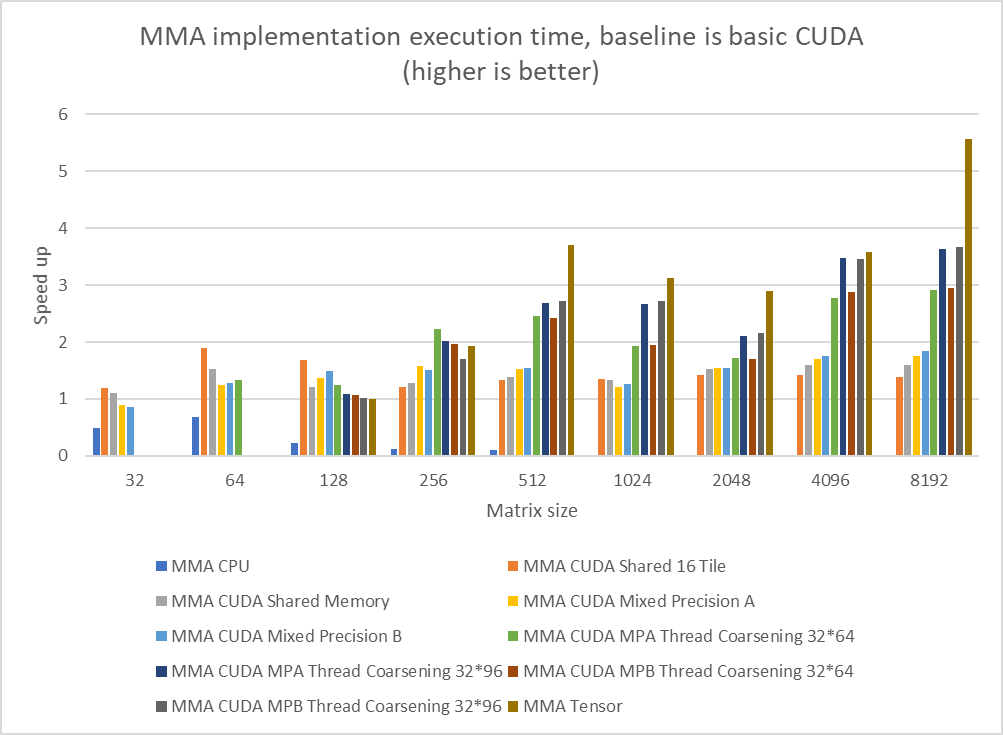
\includegraphics[scale=0.5]{figures/relative_speedup_3.png}
    \caption{Performance Comparison}
    \label{fig:performance-comparison}
  \end{figure}

  The second graph shows relative speedup to CPU of the execution of full MMA operation. 
  This include the memory allocation, the memory movement, and for some versions,
  the conversion of the data from one type to another, requiered by every mixed precision
  implementations. (See figure \ref{fig:time-comparison})
  We can see that under a matrix size of 64x64, the CPU implementation is faster than all the others
  and that it is not until a size of 256x256 that every otimplementaionher implementation beat CPU computation.
  We can also see that every mixed precision and tensor implementations are the slowest CUDA implementations
  to run even if they are the fastest to compute. This is probably caused by
  our method of converting the memory from one type to another. Therefore, these performance upgrade
  can get completely nullified by the memory management operations it requieres.


  \begin{figure}[h]
    \centering
    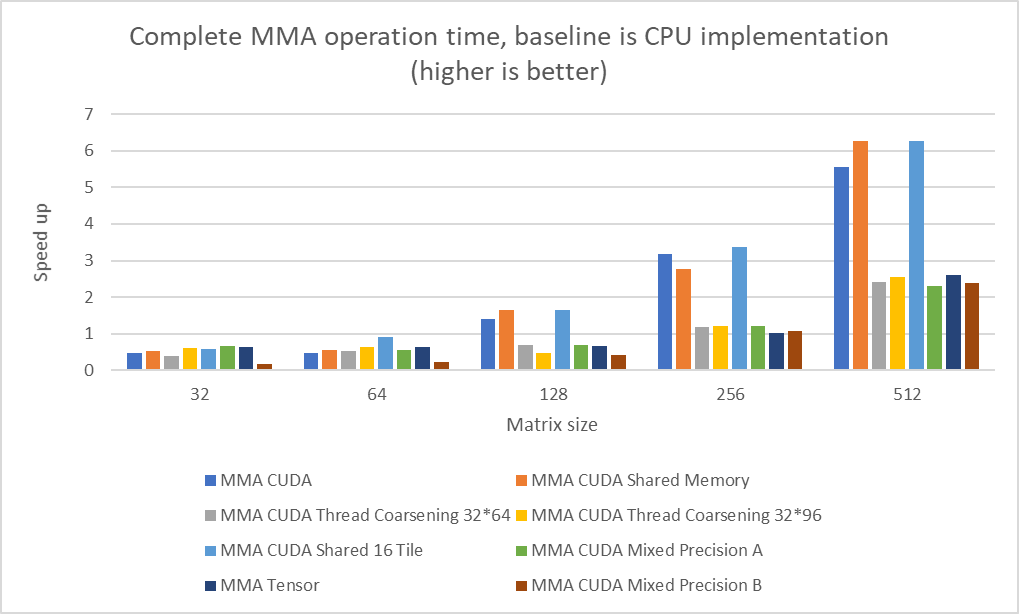
\includegraphics[scale=0.5]{figures/Tot_time_relative_speedup2.png}
    \caption{Performance Comparison total time with deallocation}
    \label{fig:time-comparison}
  \end{figure}
  
  
  \subsection{Impact of Precision}\label{sec:impact-precision}
  
  To look at the precision of our implementations we compare to the CPU how much each value differ in percentage.
  Then we sum up the values of the error and divide by the number of elements in the matrix size.

  \begin{align*}
    e_{ij} &= \frac{|d_{ij}-d_{ij}'|}{d_{ij}} \\
    \mu &= \frac{1}{n^2} \sum_{i=1}^n\sum_{j=1}^n e_{ij}
    \end{align*}
    Where $d_{ij}'$ is the output of the implementation in the $i-$th row and $j-$th column of the matrix,
    and $n$ is the matrix size.\\

  By looking at the figure~\ref{fig:precision-impact} we can see that each thread coarsening implementation (32x96)
  have an exceptionally high error of more than 25\% compared to the other implementations under a matrix size of 256x256.
  For smaller matrices the tiling is just not effective and will overlap and hence cause a big error. This is revealing that 
  our thread coarsening implementation may need some more refinement. The tensor implementation has also a high mean of error of
  more than 5\% on matrices of size 256x256.
  We also see that the error decreases with size with all of these implementations.
  This may be attributed to the number used in our testing, which is random floating point numbers between 0 and 1. 
  When conducting a test using only integers, the error is 0.
  \begin{figure}[htbp]
    \centering
    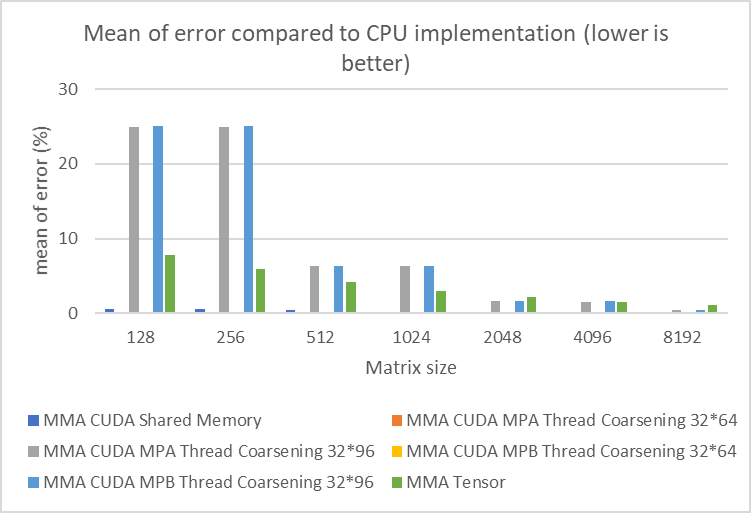
\includegraphics[scale=0.6]{figures/Mean of error compared to CPU3.png}
    \caption{Impact of Precision on mixed precision computation and tensor cores Performance}
    \label{fig:precision-impact}
  \end{figure}

  On the figure \ref{fig:precision-impact2} we can see that computing in half precision our data gives us a little more 
  impresitions, but these impresitions decrease over time, and the difference is also not that big considering how small the 
  impresition value is.

  \begin{figure}[htbp]
    \centering
    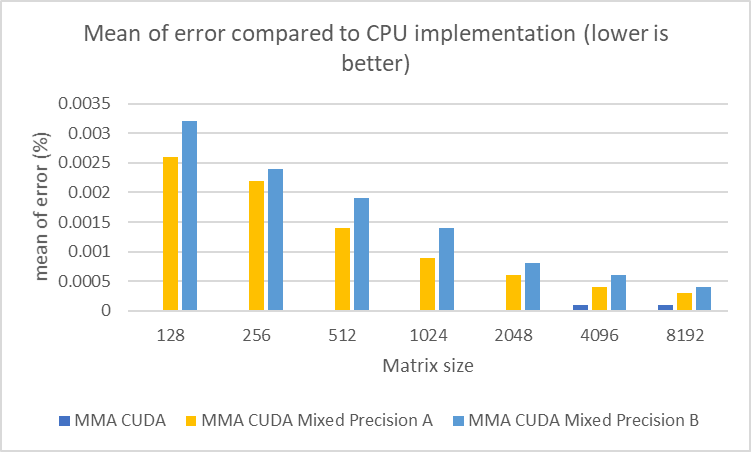
\includegraphics[scale=0.6]{figures/Mean of error MP.png}
    \caption{Impact of Precision on mixed precision computation and tensor cores Performance}
    \label{fig:precision-impact2}
  \end{figure}
  
  The results show that using mixed precision (FP16) with tensor cores can provide significant performance improvements compared to full precision (FP32).
  This is because tensor cores can process a larger number of elements simultaneously in FP16,
  leading to higher throughput. This accuracy also improves with time for the matrix sizes.
  Using FP16 then introduces a degree of numerical approximation, affecting the accuracy of the computation.
  Therefore, the choice of computing should be carefully considered based on the specific
  requirements of the application. 
  
  
  \section{Limitations and Challenges}\label{sec:limitations-challenges}
  The main limitations faced in this project was the limited information regarding how to program tensor cores.
  This led to experimenting with different setups to achieve the fastest computation possible.
  Another challenge to achieve fast computation for larger matrices with tensors are the fact that the GPU 
  only has 64Kb of memory for each work group. With the tensor, the sum of shared memory is then NxN x (16x16).
  Which corresponds to the matrix size, and the byte size of the elements in the A and B matrix. This entails that the 
  largest matrices that can fit this is of 32x32 elements of half precision.


  \section{Conclusion}\label{sec:conclusion}
  
  In this paper, we have explored the performance of NVIDIA tensor cores for matrix multiplication and accumulation operations. 
  We conducted experiments to compare the performance of tensor cores with CPU and GPU implementations, 
  considering different matrix sizes and precision settings.

  From our result we can see that tensor cores without any optimization have significantly better computational time
  than the other approaches. It is then our belief that optimizing the tensor core version would further 
  decrease the computational time. The total time comparison shows that allocation of memory has a significant
  impact on the time from input to output. Therefore using tensor cores is optimal in problen where the same data is
  handled continously, for example in convulational neural network and image processing. The error decreases
  with matrix size which can be attributed to the values we are using when testing. 

  

\bibliographystyle{IEEEtran}
\bibliography{sources}

\end{document}